\documentclass[12pt,reqno]{article}

%%%%%%%%%%%%%%%%%%%% PACKAGES %%%%%%%%%%%%%%%%%%%%

\usepackage[utf8]{inputenc}
\usepackage[all]{xy}
\usepackage[T1]{fontenc}
\usepackage[usenames, dvipsnames]{color}
\usepackage{setspace}
\usepackage{dsfont}
\usepackage{amssymb}
\usepackage{amsthm,bbm}
\usepackage{amscd}
\usepackage{amsfonts}
\usepackage{stmaryrd}
\usepackage{amsmath}
\usepackage{graphicx}
\usepackage{multicol}
\usepackage{xspace}
\usepackage{extarrows}
\usepackage{color}
\usepackage [english]{babel}
\usepackage [autostyle, english = american]{csquotes}
\usepackage[colorlinks, linktocpage, citecolor = red, linkcolor = blue]{hyperref}
\usepackage{fullpage}
\usepackage{color}
\usepackage{euler}
\usepackage{parskip}
\usepackage{tikz}

%%%%%%%%%%%%%%%%%%%% INITIALIZATION %%%%%%%%%%%%%%%%%%%%

\MakeOuterQuote{"}
\graphicspath{ {./} }

%%%%%%%%%%%%%%%%%%%% COMMANDS %%%%%%%%%%%%%%%%%%%%

\newcommand{\range}{\mathrm{range\,}}
\newcommand{\nul}{\mathrm{null\,}}
\newcommand{\spn}{\mathrm{span\,}}
\newcommand{\card}{\mathrm{cardinality}}
\newcommand{\R}{\mathbb{R}}
\newcommand{\C}{\mathbb{C}}
\newcommand{\F}{\mathbb{F}}
\newcommand{\Z}{\mathbb{Z}}
\newcommand{\bd}{\mathrm{bd\,}}
\newcommand{\divline}{\hrule\vspace{12pt}\noindent}
\newcommand{\sgn}{\mathrm{sgn}}

%%%%%%%%%%%%%%%%%%%% ENVIRONMENTS %%%%%%%%%%%%%%%%%%%%

\theoremstyle{plain}
\newtheorem{maintheorem}{Theorem}
\renewcommand*{\themaintheorem}{\Alph{maintheorem}}

\newtheorem{theorem}{Theorem}[section] 
\newtheorem{lemma}{Lemma}
\newtheorem{corollary}[theorem]{Corollary}

\theoremstyle{definition}
\newtheorem{problem}{Problem}
\newtheorem{example}[theorem]{Example}
\newtheorem{definition}[theorem]{Definition}
\newtheorem{question}[theorem]{Question}

\newtheorem*{maintheorema}{Theorem \ref{thm:main}}

%%%%%%%%%%%%%%%%%%%% TITLE-PAGE %%%%%%%%%%%%%%%%%%%%

\title{MATH 1530 Problem Set 5}
\author{Tanish Makadia\\\small{(Collaborated with Esmé and Kazuya)}}
\date{March 2023}

%%%%%%%%%%%%%%%%%%%% DOCUMENT %%%%%%%%%%%%%%%%%%%%

\begin{document}
\maketitle

%%%%%%%%%%%%%%%%%%%% PROBLEM 1 %%%%%%%%%%%%%%%%%%%%

\begin{problem} 
    Let $G$ be a finite Abelian group and let $n$ be a positive integer that is relatively prime to $|G|$.
    Prove that the mapping 
    $a \mapsto a^n$
    is an automorphism of $G$.
\end{problem}

\newpage
    
%%%%%%%%%%%%%%%%%%%% PROBLEM 2 %%%%%%%%%%%%%%%%%%%%

\begin{problem} 
    Let $G$ be a group of order $pqr$, where $p$, $q$, $r$ are distinct primes. If $H$ is a subgroup of $G$ of order $pq$ and $K$ is a subgroup of $G$ of order $qr$, prove that $|H \cap K| = q$.
\end{problem}

\begin{proof}
    We have already proven that \(H\cap K\) is a subgroup of \(G\). This implies that \(H\cap K\) is also a
    subgroup of \(H\) and \(K\). By \emph{Lagrange's Theorem}, we have that 
    \[|H\cap K|\mid |H|,|K|\implies |H\cap K|\mid pq,qr\]
    Therefore, \(|H\cap K|\) is either \(1\) or \(q\). Assume for contradiction that
    \(|H\cap K|=1\). By lemma \ref{lem:HK}, we have that
    \[|HK|=\frac{pq\cdot qr}{1}=pq^2r\]
    which is a contradiction since \(HK\) is a subset of \(G\), which implies that
    \(|HK|\leq|G|\). Therefore, we have shown that \(|H\cap K|=q\) as desired.
\end{proof}
\bigskip
\begin{lemma}
    \label{lem:HK}
    Let \(H\) and \(K\) be subgroups of a finite group \(G\). Then,
    \[|HK|=\frac{|H||K|}{|H\cap K|} \text{ where } HK=\{hk\ |\ h\in H,\ k\in K\}\]
    
    \begin{proof}
        We can separate \(HK\) into a union of left cosets of \(K\) in \(G\):
        \[HK=\bigcup_{h\in H} hK\]
        By the properties of cosets, we have that \(hK=h'K\) or \(hK\cap h'K=\emptyset\) for all
        \(h,h'\in H\). We must now determine how many of these cosets are distinct.
        
        Suppose \(hK=h'K\) for some \(h,h'\in H\). Since \(hK=h'K \Leftrightarrow h^{-1}h'\in K\), we have that
        \(h^{-1}h'=k\) for some \(k\in K\). This implies that \(k\in H\implies k\in H\cap K\).
        Additionally, \(h'=hk\). Thus, there are \(|H\cap K|\) ways to create the same coset for each \(h'\in H\)
        (by \emph{Cayley's Theorem}, we know that each \(k\in H\cap K\) has exactly one corresponding \(h\in H\) such that
        \(hk=h'\)). Therefore, the number of distinct cosets \(hK\) where \(h\in H\) is \(|H|/|H\cap K|\).

        Since \(|hK|=|h'K|\) for all \(h,h'\in H\), the number of elements in each coset is \(|hK|=|K|\). Therefore,
        the cardinality of \(HK\) equals the number of distinct cosets times the number of distinct elements in each coset, giving us
        \[|HK|=\frac{|H||K|}{|H\cap K|}\]
    \end{proof}
\end{lemma}

\newpage
    
%%%%%%%%%%%%%%%%%%%% PROBLEM 3 %%%%%%%%%%%%%%%%%%%%

\begin{problem} 
    Calculate the order of the group of rotations of a regular dodecahedron:
    \begin{center}
        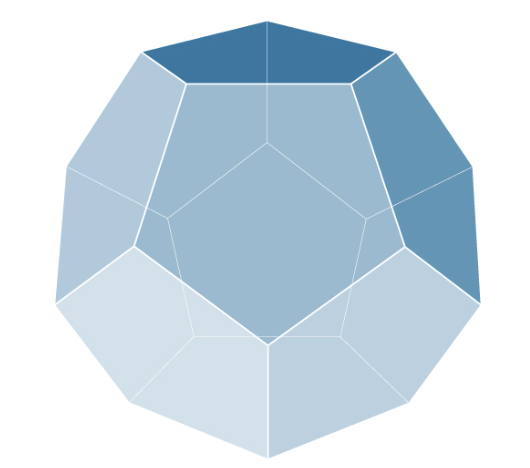
\includegraphics[height = 1.6 in]{Screenshot 2023-03-03 at 1.12.39 PM.png}
    \end{center}
\end{problem}

\newpage
    
%%%%%%%%%%%%%%%%%%%% PROBLEM 4 %%%%%%%%%%%%%%%%%%%%

\begin{problem} 
    Determine the number of cyclic subgroups of order 15 in $\mathbb{Z}_{90} \oplus \mathbb{Z}_{36}$.
\end{problem}

\newpage
    
%%%%%%%%%%%%%%%%%%%% PROBLEM 5 %%%%%%%%%%%%%%%%%%%%

\begin{problem} 
    Let $p$ and $q$ be odd primes and let $m$ and $n$ be positive integers. Prove that $U(p^m) \oplus U(q^n)$ is not cyclic. [hint: read the book to find a useful result we didn't cover in class]
\end{problem}

\end{document}